%%%%%%%%%%%%%%%%%%%%%%%%%%%%%%%%%%%%%%%%%
% Journal Article
% LaTeX Template
% Version 1.3 (9/9/13)
%
% This template has been downloaded from:
% http://www.LaTeXTemplates.com
%
% Original author:
% Frits Wenneker (http://www.howtotex.com)
%
% License:
% CC BY-NC-SA 3.0 (http://creativecommons.org/licenses/by-nc-sa/3.0/)
%
%%%%%%%%%%%%%%%%%%%%%%%%%%%%%%%%%%%%%%%%%
%----------------------------------------------------------------------------------------
%       PACKAGES AND OTHER DOCUMENT CONFIGURATIONS
%----------------------------------------------------------------------------------------
\documentclass[paper=letter, fontsize=12pt]{article}
\newcommand{\RNum}[1]{\uppercase\expandafter{\romannumeral #1\relax}} %Para numeros romanos
\usepackage[english]{babel} % English language/hyphenation
\usepackage{amsmath,amsfonts,amsthm} % Math packages
\usepackage{tikz}%para mapa de karnaugh
\usepackage[utf8]{inputenc}
\usepackage{float}
\usepackage{lipsum} % Package to generate dummy text throughout this template
\usepackage{blindtext}
\usepackage{listings} %para codigo
\usepackage{graphicx} 
\usepackage{amsmath}
\usepackage{xcolor}
\usepackage[export]{adjustbox}

\usepackage{listings}
\usepackage{color} %red, green, blue, yellow, cyan, magenta, black, white
\definecolor{mygreen}{RGB}{28,172,0} % color values Red, Green, Blue
\definecolor{mylilas}{RGB}{170,55,241}

\definecolor{mGreen}{rgb}{0,0.6,0}
\definecolor{mGray}{rgb}{0.5,0.5,0.5}
\definecolor{mPurple}{rgb}{0.58,0,0.82}
\definecolor{backgroundColour}{rgb}{0.95,0.95,0.92}

\lstdefinestyle{CStyle}{
    backgroundcolor=\color{backgroundColour},   
    commentstyle=\color{mGreen},
    keywordstyle=\color{magenta},
    numberstyle=\tiny\color{mGray},
    stringstyle=\color{mPurple},
    basicstyle=\footnotesize,
    breakatwhitespace=false,         
    breaklines=true,                 
    captionpos=b,                    
    keepspaces=true,                 
    numbers=left,                    
    numbersep=5pt,                  
    showspaces=false,                
    showstringspaces=false,
    showtabs=false,                  
    tabsize=2,
    language=C
}

\lstset{language=Matlab,%
    %basicstyle=\color{red},
    breaklines=true,%
    morekeywords={matlab2tikz},
    keywordstyle=\color{blue},%
    morekeywords=[2]{1}, keywordstyle=[2]{\color{black}},
    identifierstyle=\color{black},%
    stringstyle=\color{mylilas},
    commentstyle=\color{mygreen},%
    showstringspaces=false,%without this there will be a symbol in the places where there is a space
    numbers=left,%
    numberstyle={\tiny \color{black}},% size of the numbers
    numbersep=9pt, % this defines how far the numbers are from the text
    emph=[1]{for,end,break},emphstyle=[1]\color{red}, %some words to emphasise
    %emph=[2]{word1,word2}, emphstyle=[2]{style},    
}



\usepackage{caption}
\usepackage{subcaption}

\usepackage[sc]{mathpazo} % Use the Palatino font
\usepackage[T1]{fontenc} % Use 8-bit encoding that has 256 glyphs
\linespread{1.05} % Line spacing - Palatino needs more space between lines
\usepackage{microtype} % Slightly tweak font spacing for aesthetics
\usepackage[hmarginratio=1:1,top=32mm,columnsep=20pt]{geometry} % Document margins
\usepackage{multicol} % Used for the two-column layout of the document
%\usepackage[hang, small,labelfont=bf,up,textfont=it,up]{caption} % Custom captions under/above floats in tables or figures
\usepackage{booktabs} % Horizontal rules in tables
\usepackage{float} % Required for tables and figures in the multi-column environment - they need to be placed in specific locations with the [H] (e.g. \begin{table}[H])
\usepackage{hyperref} % For hyperlinks in the PDF
\usepackage{lettrine} % The lettrine is the first enlarged letter at the beginning of the text
\usepackage{paralist} % Used for the compactitem environment which makes bullet points with less space between them
\usepackage{abstract} % Allows abstract customization
\renewcommand{\abstractnamefont}{\normalfont\bfseries} % Set the "Abstract" text to bold
\renewcommand{\abstracttextfont}{\normalfont\small\itshape} % Set the abstract itself to small italic text
\usepackage{titlesec} % Allows customization of titles
\usetikzlibrary{matrix,calc} %para mapa de karnaugh
\renewcommand\thesection{\Roman{section}} % Roman numerals for the sections
\renewcommand\thesubsection{\Roman{subsection}} % Roman numerals for subsections
%isolated term
%#1 - Optional. Space between node and grouping line. Default=0
%#2 - node
%#3 - filling color
\newcommand{\implicantsol}[3][0]{
    \draw[rounded corners=3pt, fill=#3, opacity=0.3] ($(#2.north west)+(135:#1)$) rectangle ($(#2.south east)+(-45:#1)$);
    }


%internal group
%#1 - Optional. Space between node and grouping line. Default=0
%#2 - top left node
%#3 - bottom right node
%#4 - filling color
\newcommand{\implicant}[4][0]{
    \draw[rounded corners=3pt, fill=#4, opacity=0.3] ($(#2.north west)+(135:#1)$) rectangle ($(#3.south east)+(-45:#1)$);
    }

%group lateral borders
%#1 - Optional. Space between node and grouping line. Default=0
%#2 - top left node
%#3 - bottom right node
%#4 - filling color
\newcommand{\implicantcostats}[4][0]{
    \draw[rounded corners=3pt, fill=#4, opacity=0.3] ($(rf.east |- #2.north)+(90:#1)$)-| ($(#2.east)+(0:#1)$) |- ($(rf.east |- #3.south)+(-90:#1)$);
    \draw[rounded corners=3pt, fill=#4, opacity=0.3] ($(cf.west |- #2.north)+(90:#1)$) -| ($(#3.west)+(180:#1)$) |- ($(cf.west |- #3.south)+(-90:#1)$);
}

%group top-bottom borders
%#1 - Optional. Space between node and grouping line. Default=0
%#2 - top left node
%#3 - bottom right node
%#4 - filling color
\newcommand{\implicantdaltbaix}[4][0]{
    \draw[rounded corners=3pt, fill=#4, opacity=0.3] ($(cf.south -| #2.west)+(180:#1)$) |- ($(#2.south)+(-90:#1)$) -| ($(cf.south -| #3.east)+(0:#1)$);
    \draw[rounded corners=3pt, fill=#4, opacity=0.3] ($(rf.north -| #2.west)+(180:#1)$) |- ($(#3.north)+(90:#1)$) -| ($(rf.north -| #3.east)+(0:#1)$);
}

%group corners
%#1 - Optional. Space between node and grouping line. Default=0
%#2 - filling color
\newcommand{\implicantcantons}[2][0]{
    \draw[rounded corners=3pt, opacity=.3] ($(rf.east |- 0.south)+(-90:#1)$) -| ($(0.east |- cf.south)+(0:#1)$);
    \draw[rounded corners=3pt, opacity=.3] ($(rf.east |- 8.north)+(90:#1)$) -| ($(8.east |- rf.north)+(0:#1)$);
    \draw[rounded corners=3pt, opacity=.3] ($(cf.west |- 2.south)+(-90:#1)$) -| ($(2.west |- cf.south)+(180:#1)$);
    \draw[rounded corners=3pt, opacity=.3] ($(cf.west |- 10.north)+(90:#1)$) -| ($(10.west |- rf.north)+(180:#1)$);
    \fill[rounded corners=3pt, fill=#2, opacity=.3] ($(rf.east |- 0.south)+(-90:#1)$) -|  ($(0.east |- cf.south)+(0:#1)$) [sharp corners] ($(rf.east |- 0.south)+(-90:#1)$) |-  ($(0.east |- cf.south)+(0:#1)$) ;
    \fill[rounded corners=3pt, fill=#2, opacity=.3] ($(rf.east |- 8.north)+(90:#1)$) -| ($(8.east |- rf.north)+(0:#1)$) [sharp corners] ($(rf.east |- 8.north)+(90:#1)$) |- ($(8.east |- rf.north)+(0:#1)$) ;
    \fill[rounded corners=3pt, fill=#2, opacity=.3] ($(cf.west |- 2.south)+(-90:#1)$) -| ($(2.west |- cf.south)+(180:#1)$) [sharp corners]($(cf.west |- 2.south)+(-90:#1)$) |- ($(2.west |- cf.south)+(180:#1)$) ;
    \fill[rounded corners=3pt, fill=#2, opacity=.3] ($(cf.west |- 10.north)+(90:#1)$) -| ($(10.west |- rf.north)+(180:#1)$) [sharp corners] ($(cf.west |- 10.north)+(90:#1)$) |- ($(10.west |- rf.north)+(180:#1)$) ;
}



\titleformat{\section}[block]{\large\scshape\centering}{\thesection.}{1em}{} % Change the look of the section titles
\titleformat{\subsection}[block]{\large}{\thesubsection.}{1em}{} % Change the look of the section titles
\newcommand{\horrule}[1]{\rule{\linewidth}{#1}} % Create horizontal rule command with 1 argument of height
\usepackage{fancyhdr} % Headers and footers
\pagestyle{fancy} % All pages have headers and footers
\fancyhead{} % Blank out the default header
\fancyfoot{} % Blank out the default footer

\lhead[C]{FCEFyN-UNC } % Custom header text
\rhead{
\includegraphics[scale=0.2]{header_unc.jpg}}
\fancyfoot[RO,LE]{\thepage} % Custom footer text
%----------------------------------------------------------------------------------------
%       TITLE SECTION
%----------------------------------------------------------------------------------------
\title{\bigskip \bigskip \bigskip \bigskip \vspace{-15mm}\fontsize{28pt}{12pt}\selectfont\textbf{\textcolor{teal}{Electrónica Digital \RNum{3}}}\\
\bigskip \bigskip \fontsize{18pt}{10pt}\selectfont\textbf{\textcolor{violet}{Trabajo final: SIMON GAME}}} % Article title
\author{
\large
{\textsc{Casabella Martin, 39.694.763 }}\\[2mm]
\bigskip
\textsc{Zimmel Ezequiel José, 33.382.573 }\\[2mm]
\bigskip
\textsc{\textbf{\textcolor{orange}{GRUPO 12}}}\\[2mm]
}
\date{}


%Empty Karnaugh map 4x4
\newenvironment{Karnaugh}%
{
\begin{tikzpicture}[baseline=(current bounding box.north),scale=0.8]
\draw (0,0) grid (4,4);
\draw (0,4) -- node [pos=0.7,above right,anchor=south west] {AB} node [pos=0.7,below left,anchor=north east] {CZ} ++(135:1);
%
\matrix (mapa) [matrix of nodes,
        column sep={0.8cm,between origins},
        row sep={0.8cm,between origins},
        every node/.style={minimum size=0.3mm},
        anchor=8.center,
        ampersand replacement=\&] at (0.5,0.5)
{
                       \& |(c00)| 00         \& |(c01)| 01         \& |(c11)| 11         \& |(c10)| 10         \& |(cf)| \phantom{00} \\
|(r00)| 00             \& |(0)|  \phantom{0} \& |(1)|  \phantom{0} \& |(3)|  \phantom{0} \& |(2)|  \phantom{0} \&                     \\
|(r01)| 01             \& |(4)|  \phantom{0} \& |(5)|  \phantom{0} \& |(7)|  \phantom{0} \& |(6)|  \phantom{0} \&                     \\
|(r11)| 11             \& |(12)| \phantom{0} \& |(13)| \phantom{0} \& |(15)| \phantom{0} \& |(14)| \phantom{0} \&                     \\
|(r10)| 10             \& |(8)|  \phantom{0} \& |(9)|  \phantom{0} \& |(11)| \phantom{0} \& |(10)| \phantom{0} \&                     \\
|(rf) | \phantom{00}   \&                    \&                    \&                    \&                    \&                     \\
};
}%
{
\end{tikzpicture}
}

%Defines 8 or 16 values (0,1,X)
\newcommand{\contingut}[1]{%
\foreach \x [count=\xi from 0]  in {#1}
     \path (\xi) node {\x};
}

%Places 1 in listed positions
\newcommand{\minterms}[1]{%
    \foreach \x in {#1}
        \path (\x) node {1};
}

%Places 0 in listed positions
\newcommand{\maxterms}[1]{%
    \foreach \x in {#1}
        \path (\x) node {0};
}

%Places X in listed positions
\newcommand{\indeterminats}[1]{%
    \foreach \x in {#1}
        \path (\x) node {X};
}



%----------------------------------------------------------------------------------------
\begin{document}
\maketitle % Insert title
\thispagestyle{fancy} % All pages have headers and footers

\bigskip
\bigskip
\section{\textbf{Juego de memoria SIMON}}

SIMON es un juego electrónico que desafía la memoria. El usuario básicamente tiene que repetir la secuencia mostrada en el tablero para progresar al siguiente nivel. En la presente implementación del juego, el usuario puede elegir entre 3 modos de juego:\\
\begin{enumerate}
\item 	Modo Progresivo o Clásico, donde el juego reutiliza el nivel anterior como inicio del siguiente nivel antes de añadir un paso aleatorio al final;
\item         Modo Inverso: se debe proceder a realizar la secuencia generada y mostrada pero al revés
\item 	Modo Aleatorio, donde cada nivel del juego produce una nueva secuencia aleatoria, cada paso más largo que el anterior;
\item 	Modo Multijugador, donde cada usuario añade una nota a la secuencia, siendo el primero en equivocarse el perdedor.
\end{enumerate}

A su vez, como mando de juego, el usuario puede optar por manejarse con botones o como alternativa, una palanca de mando o $joystick$.\\
\clearpage

\section{\textbf{Requerimientos}}

\begin{itemize}
\item Selección de modo de juego.
\item Selección de dificultad.
\item Selección de cantidad de notas a tocar.
\item Generación aleatoria de secuencia.
\item Activación sonora y visual de la nota.
\item Activación de las notas a través del movimiento de un giróscopo.
\item Mantener estado de la secuencia de juego.
\item Despliegue de estado del juego por pantalla LCD.
\item Comunicación serial para modo multijugador.
\end{itemize}

\hfill \break

\section{\textbf{Especificaciones}}
\begin{itemize}
\item Uso de microcontrolador LPC1769
\item Codificación en C.
\item Ingreso de valores mediante pulsadores.
\item Aviso de nota tocada mediante sonido (Buzzer piezoeléctrico) e iluminación (LED).
\item Utilización de LCD 16x2 ‘1602A’.
\item Empleo de joystick, como mando alternatico.
\item Comunicación serie mediantes pines específicos de la placa de desarrollo.
\end{itemize}

\clearpage

\section{\textbf{Esquemático del diseño elaborado}}
\begin{figure}[H]
  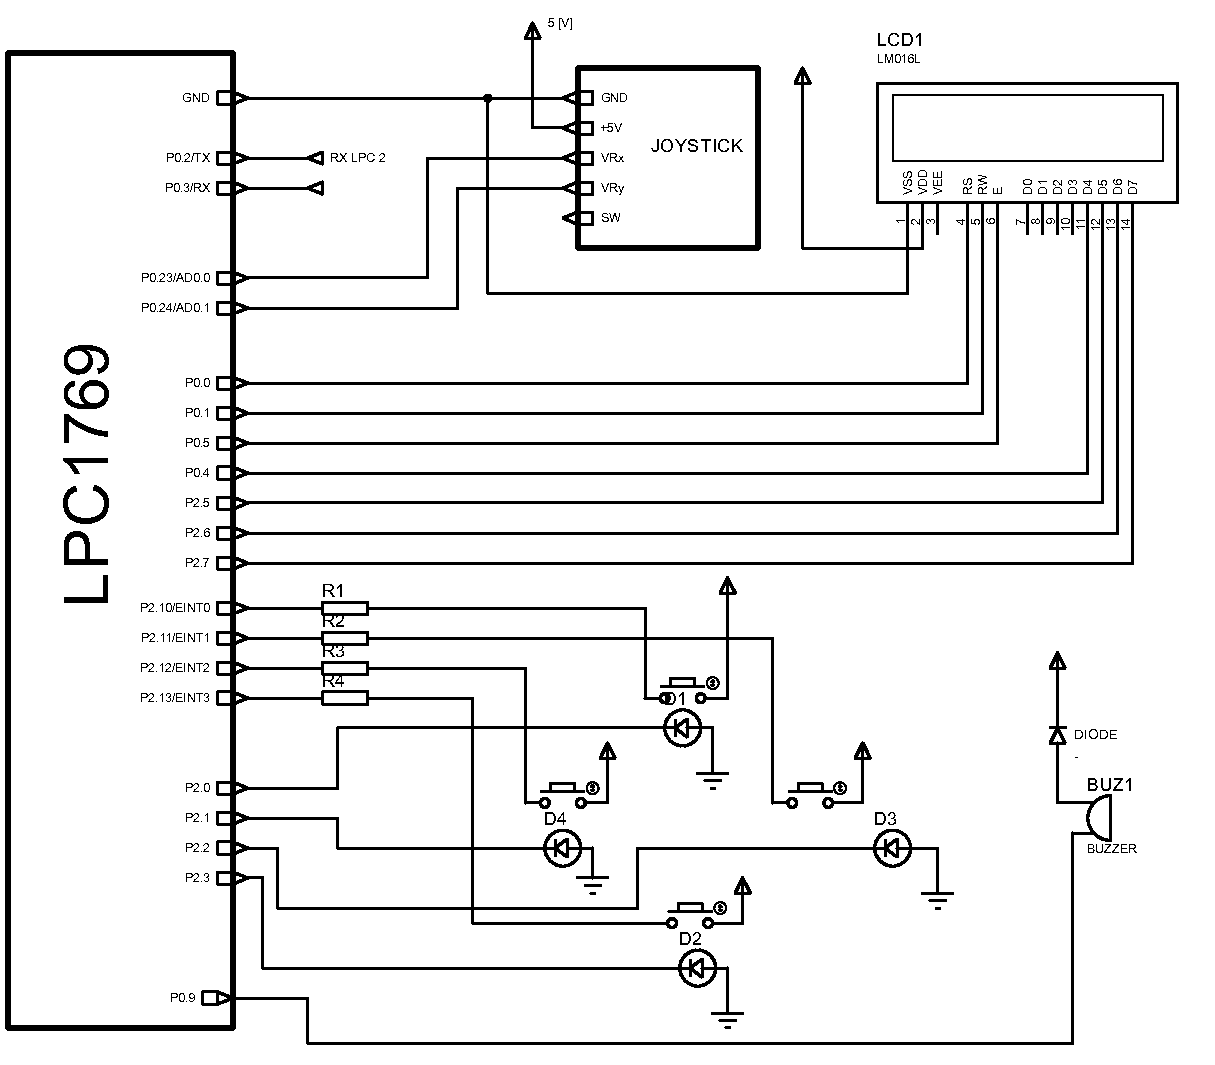
\includegraphics[scale=0.85]{PROJ.pdf}
  \caption{Diagrama circuital}
 \end{figure}

\hfill \break
Este esquema se replica en la otra placa utilizada para probar el modo multijugador. \\

Se ve en el diagrama, que el transmisor del modulo UART, se conecta al receptor de la otra placa, y el receptor al transmisor, para efectuar la comunicacion. \\



\subsection{Asignación de pines en detalle}
\begin{table}[H]
\centering
%\begin{tabular}{@{\hskip 1in}{}||@{}ll@{}}
\begin{tabular}{l@{\hskip 0.5in}c@{\hskip 0.5in}c}
\toprule
Periferico & Pin del periferico \hfill \hfill \hfill & Pin de la placa asignado \\ \midrule
 LCD & RS   &  P0.0 \\
  & RW   & P0.1 \\
 & EN   & P0.5 \\
 & D4   & P0.4 \\
 & D5   & P2.5 \\
 & D6   & P2.6 \\
 & D7   & P2.7 \\ \bottomrule
 Joystick & VRx  &  P0.23 \\
  & VRy   & P0.24 \\\bottomrule
\end{tabular}
\caption{Asignación de pines para el Joystick y el LCD}
\label{PINES}
\end{table}

\hfill \break

\begin{table}[H]
\centering
%\begin{tabular}{@{\hskip 1in}{}ll@{}}
\begin{tabular}{l@{\hskip 0.5in}c@{\hskip 0.5in}c}
\toprule
Periferico \hfill \hfill & Pin de la placa asignado \\ \midrule
Pulsadores &   P2.10/EINT0\\
 &  P2.11/EINT1 \\
 &   P2.12/EINT2 \\
 &   P2.13/ EINT3  \\ \bottomrule
Buzzer &  P0.9\\ \bottomrule
LEDS &  P2.0 \\ 
 &  P2.1 \\
 &  P2.2\\
 &  P2.3\\ \bottomrule
 UART  & P0.2 \\
  &  P0.3 \\ \bottomrule
    \end{tabular}
\caption{Asignación de pines para pulsadores, leds, y modulo UART}
\label{PINES}
\end{table}
\clearpage

\section{\textbf{Código empleado}}

Se elaboraron los siguientes archivos (código fuente en C) y headers:\\
\begin{figure}[H]
  \includegraphics[scale=0.85]{Jerarquia.jpg}
  \caption{Archivos : códigos fuentes y headers}
 \end{figure}
 
 \hfill \break
 \hfill \break 

 
\subsection{\textbf{TP\_FINAL\_ED3.c}}
 Programa principal: arranca el juego mostrando en el LCD al usuario que modos de juego puede elegir, y en función al ingreso del usuario, ejecuta las funciones de un modo u otro. \\
 Al finalizar, le indica al usuario si gano o perdió a través del LCD y una secuencia de luces indicativas. Luego vuelve a mostrar las opciones de modos de juego para que el usuario pueda volver a jugar si así lo desea.\\
 Incluye los siguientes archivos headers:
 \begin{itemize}
 \item $configuracion.h$
 \item $leds.h$
 \item$simon.h$
 \item$lcd.h$
 \end{itemize}
  
\clearpage
 \begin{lstlisting}[style=CStyle]
#ifdef __USE_CMSIS
#include "LPC17xx.h"
#endif

#include <cr_section_macros.h>

#include <stdio.h>
#include "configuracion.h"
#include "leds.h"
#include "simon.h"
#include "lcd.h"

int
main (void)
{
  int juego = 0, nivel = 0, exito = 0;

  clearPulsador ();
  clear_SELMODE ();
  perifericos_Init ();
  leds_Init ();
  Lcd_Init (LCD_RS, LCD_RW, LCD_EN, LCD_D4, LCD_D5, LCD_D6, LCD_D7);
  Lcd_Show ("SIMON", 1, 7, 0, 0);
  Lcd_Show ("--EDIII--", 2, 5, 0, 0);
  simon_Init (1000000);

  while (1)
    {
      Lcd_Show ("1) 4", 1, 1, 1, 0);
      Lcd_Show ("2) 8", 1, 10, 0, 0);
      Lcd_Show ("3) 12", 2, 1, 0, 0);
      Lcd_Show ("4) 16", 2, 10, 0, 0);
      while (!nivel)
	{
	  nivel = getPulsador ();
	  LPC_SC->EXTINT |= ~0;
	  retardo (500000);
	}
      clearPulsador ();
      clear_SELMODE ();
      Lcd_Show ("1)Clasi", 1, 1, 1, 0);
      Lcd_Show ("2)Inver", 1, 10, 0, 0);
      Lcd_Show ("3)Avanz", 2, 1, 0, 0);
      Lcd_Show ("4)Multi", 2, 10, 0, 0);
      juego = 0;
      while (!juego)
	{
	  juego = getPulsador ();
	  LPC_SC->EXTINT |= ~0;
	  retardo (500000);
	}

      switch (juego)
	{
	case (1):
	  Lcd_Show ("MODO CLASICO", 1, 4, 1, 2500000);
	  Lcd_Show ("3", 2, 9, 0, 2500000);
	  Lcd_Show ("2", 2, 9, 0, 2500000);
	  Lcd_Show ("1", 2, 9, 0, 2500000);
	  Lcd_Show ("A JUGAR!", 1, 6, 1, 5000000);
	  modo_1 (nivel, &exito);
	  break;
	case (2):
	  Lcd_Show ("MODO INVERSO", 1, 4, 1, 2500000);
	  Lcd_Show ("3", 2, 9, 0, 2500000);
	  Lcd_Show ("2", 2, 9, 0, 2500000);
	  Lcd_Show ("1", 2, 9, 0, 2500000);
	  Lcd_Show ("A JUGAR!", 1, 6, 1, 5000000);
	  modo_2 (nivel, &exito);
	  break;
	case (3):
	  printf("Modo avanzado JOYSTICK: \n");
	  Lcd_Show ("MODO AVANZADO", 1, 3, 1, 2500000);
	  Lcd_Show ("3", 2, 9, 0, 2500000);
	  Lcd_Show ("2", 2, 9, 0, 2500000);
	  Lcd_Show ("1", 2, 9, 0, 2500000);
	  Lcd_Show ("A JUGAR!", 1, 6, 1, 5000000);
	  modo_3 (nivel, &exito);
	  break;
	case (4):
	  Lcd_Show ("MULTIJUGADOR", 1, 4, 1, 2500000);
	  Lcd_Show ("3", 2, 9, 0, 2500000);
	  Lcd_Show ("2", 2, 9, 0, 2500000);
	  Lcd_Show ("1", 2, 9, 0, 2500000);
	  printf("\n Entre en modo 4 \n");
	  modo_4 (nivel, &exito);
	  break;
	}

      if (juego != 4)
	{
	  if (exito)
	    {
	      Lcd_Show ("GANASTE!", 1, 5, 1, 0);
	      simon_SUCCESS ();
	    }
	  else
	    {
	      Lcd_Show ("PERDISTE!", 1, 5, 1 , 0);
	      simon_FAIL ();
	    }
	}
      clear_SELMODE ();
      nivel = 0;
      juego = 0;
      clearPulsador ();

      Lcd_Show ("A JUGAR!", 1, 6, 1, 0);
      simon_Init (500000);

    }

}

\end{lstlisting}
  
 \clearpage
 
 \subsection{\textbf{configuracion.c}}
 Este archivo es el encargado de configurar cada periférico utilizado (ADC, timer, systick, UART), junto con las interrupciones y el puerto de propósito general. \\
 Incluye solamente el header $configuracion.h$. Se anexan las funciones empleadas:\\
 
 \begin{lstlisting}[style=CStyle]
#include "configuracion.h"

uint32_t volatile * const STCTRL = (uint32_t *) AddrSTCTRL;
uint32_t volatile * const STRELOAD = (uint32_t *) AddrSTRELOAD;

uint32_t RELOAD[4] =
  { 103370, 167404, 254545, 356759 };	//{Amarillo, Verde, Rojo, Azul}

/**
 * @brief  Configuracion de los pines a ser utilizados
 */
void
gpioConfig (void)
{
  LPC_PINCON->PINSEL0 |= (1 << 4);				//Funcion del Pin0.2	TX
  LPC_PINCON->PINSEL0 |= (1 << 6);				//FUncion del Pin0.3	RX
  LPC_PINCON->PINSEL1 |= (1 << 14);			//Funcion del Pin0.23  AD0.0
  LPC_PINCON->PINSEL1 |= (1 << 16);			//Funcion del Pin0.24  AD0.1
  LPC_PINCON->PINSEL1 |= (1 << 18);			//Funcion del Pin0.25  AD0.2
  LPC_PINCON->PINSEL4 |= (0b00 << 0);			//Funcion del Pin2.0 ESTA COMO GPIO, para PWM1.1 poner 0b10
  LPC_PINCON->PINSEL4 |= (0b00 << 2);			//Funcion del Pin2.1 ESTA COMO GPIO, para PWM1.2 poner 0b10
  LPC_PINCON->PINSEL4 |= (0b00 << 4);	                //Funcion del Pin2.2 ESTA COMO GPIO, para PWM1.3 poner 0b10
  LPC_PINCON->PINSEL4 |= (0b00 << 6);	     	        //Funcion del Pin2.3 ESTA COMO GPIO, para PWM1.4 poner 0b10
  LPC_PINCON->PINSEL4 |= (1 << 20);			//Funcion del Pin2.10: EINT0
  LPC_PINCON->PINSEL4 |= (1 << 22);			//Funcion del Pin2.11: EINT1
  LPC_PINCON->PINSEL4 |= (1 << 24);			//Funcion del Pin2.12: EINT2
  LPC_PINCON->PINSEL4 |= (1 << 26);			//Funcion del Pin2.12: EINT3
  LPC_PINCON->PINMODE1 |= (1 << 15);			//Pin0.23 entrada analogica
  LPC_PINCON->PINMODE1 |= (1 << 17);			//Pin0.24 entrada analogica
  LPC_PINCON->PINMODE1 |= (1 << 19);			//Pin0.25 entrada analogica
  LPC_PINCON->PINMODE4 |= (0b11 << 20);		//Pin2.10 Pull-down
  LPC_PINCON->PINMODE4 |= (0b11 << 22);		//Pin2.11 Pull-down
  LPC_PINCON->PINMODE4 |= (0b11 << 24);		//Pin2.12 Pull-down
  LPC_PINCON->PINMODE4 |= (0b11 << 26);		//Pin2.12 Pull-down
  //LPC_GPIO2->FIOMASK2 |= ();
  LPC_GPIO0->FIODIR |= (1 << 9);						//Pin0.9 como salida
  LPC_GPIO2->FIODIR |= (1 << 0 | 1 << 1 | 1 << 2 | 1 << 3);	//Pines 2.0/2.1/2.2/2.3 como salida
  LPC_GPIO0->FIOMASK = 0;
  LPC_GPIO0->FIOCLR |= (1 << 9);						//Bajamos salida del tono
}

/**
 * @brief   Configura los TIMERs
 */
void
timerConfig (void)
{
  //--------------TIMER0---------------
  LPC_TIM0->MR0 = 6250000;			//Match para interrupcion cada 625ms
  LPC_TIM0->MCR |= 0b11;			//Match0 interrupcion y reinicio del TC
  LPC_TIM0->TCR &= ~1;				//Deshabilitamos el contador
  LPC_TIM0->TCR |= (1 << 1);			//Reseteamos el TC y PC
  LPC_TIM0->TCR &= ~(1 << 1);		//Salimos del estado Reset
  LPC_TIM0->IR |= ~0;				//Bajamos banderas de interrupcion pendientes
  
  //--------------TIMER1---------------
  LPC_TIM1->MR0 = 10000000;			//Match para interrupcion cada 1s
  LPC_TIM1->MCR |= 0b11;			//Match0 interrupcion y reinicio del TC
  LPC_TIM1->TCR &= ~1;				//Deshabilitamos el contador
  LPC_TIM1->TCR |= (1 << 1);			//Reseteamos el TC y PC
  LPC_TIM1->TCR &= ~(1 << 1);		//Salimos del estado Reset
  LPC_TIM1->IR |= ~0;			       //Bajamos banderas de interrupcion pendientes
 
}

/**
 * @brief   Configura las interrupciones Externas
 */
void
eintConfig (void)
{
  //--------------EINT0---------------
  LPC_SC->EXTMODE |= 1;					//EINT0 sensible por flanco
  LPC_SC->EXTPOLAR |= 1;				//Flanco ascendente
  //--------------EINT1---------------
  LPC_SC->EXTMODE |= (1 << 1);			//EINT1 sensible por flanco
  LPC_SC->EXTPOLAR |= (1 << 1);			//Flanco ascendente
  //--------------EINT2---------------
  LPC_SC->EXTMODE |= (1 << 2);			//EINT2 sensible por flanco
  LPC_SC->EXTPOLAR |= (1 << 2);			//Flanco ascendente
  //--------------EINT3---------------
  LPC_SC->EXTMODE |= (1 << 3);			//EINT3 sensible por flanco
  LPC_SC->EXTPOLAR |= (1 << 3);			//Flanco ascendente
}

/**
 * @brief   Configura la comunicacion Serie UART
 */

void
uartConfig (void)
{
  LPC_SC -> PCONP  |= 1<<3;		//Encendemos periferico
  LPC_UART0->LCR |= (1 << 7);		//On DLAB
  LPC_UART0->DLL = 130;			 //PCLK 20Mhz -> 9600BR DLL en 130, DLM en 0
  LPC_UART0->DLM = 0;
  LPC_UART0->LCR &= ~(1 << 7);	 //OFF DLAB, para poder seguir cfg
  //LPC_UART0->FCR |= 1;			 // 1 Con fifo, 0 (defecto) Sin fifo
  LPC_UART0->LCR |= (0b11);		//8bits
  LPC_UART0->IER |= 1;			//Interrupcion por recepcion de datos
}

/**
 * @brief   Configura el ADC para el uso del STICK
 */
void
adcConfig (void)
{
  LPC_ADC->ADCR |= 0b11;		//Canales a muestrear AD0.0, AD0.1
  //LPC_ADC->ADCR |= (0b0 << 15);	//Divisor para el clock de periferico
  LPC_ADC->ADCR &= ~(1 << 16);	//OFF Burst
  LPC_ADC->ADCR |= (1 << 21);		//ADC operacional
  LPC_ADC->ADINTEN &= ~(1 << 8);	//Deshabilitamos interrupcion por ADC
}


/**
 * @brief    Realiza la Habilitacion de los perifericos, la configuracion de su
 * 	       frecuencia y luego habilita las interrupciones de los perifericos
 */
void
nvic_sysConfig (uint8_t i)
{
  if (i == 0)
    {
      *STCTRL &= ~(1 | (1 << 1));		//Deshabilitos cuenta e interrupcion de SysTick
      LPC_SC->PCONP |= (1 << 12);		//Activamos periferico ADC
     	
      LPC_SC->PCLKSEL0 |= (0b11 << 24);	//ADC clock = 1/8 CPU clock
      LPC_SC->PCLKSEL0 |= (0b11 << 2);	//TIMER0 clock = 1/8 CPU clock
      LPC_SC->PCLKSEL0 |= (0b11 << 4);	//TIMER1 clock = 1/8 CPU clock
      LPC_SC->PCLKSEL0 |= (0b11 << 12);	 //PWM clock = 1/8 CPU clock
      *STCTRL |= (1 << 2);
      *STRELOAD = RELOAD[0] / 2;
      i = 1;
    }
  else
    {
      LPC_SC->EXTINT |= ~0;		//Bajo banderas de interrupcion EINT
      //Habilitamos las interrupciones
      NVIC_EnableIRQ (EINT0_IRQn);
      NVIC_EnableIRQ (EINT1_IRQn);
      NVIC_EnableIRQ (EINT2_IRQn);
      NVIC_EnableIRQ (EINT3_IRQn);
      NVIC_EnableIRQ (ADC_IRQn);
      NVIC_EnableIRQ (TIMER0_IRQn);
      NVIC_EnableIRQ (TIMER1_IRQn);

      LPC_ADC->ADCR |= (1 << 16);		//Conversion Burst ON
      //*STCTRL |= (1 << 0) | (1 << 1);	//Cuenta e interrupcion de SysTick habilitadas
      i = 0;
    }
}

/*
 * Ajusta la carga del SysTick para generar un tono en particular
 * y habilita su cuenta e interrupcion.
 */

void
setTono (uint32_t freq)
{
  *STRELOAD = freq;
  *STCTRL |= (1 << 0) | (1 << 1);
}

/*
 * Deshabilita la cuenta e interrupcion del SysTick.
 */

void
sysTick_OFF (void)
{
  *STCTRL &= ~(1 | (1 << 1));
}


/*
* Setea el tiempo de interrupcion del timer, con el valor pasado como parametro
*/
void
setTiempo (uint8_t timer, uint32_t tiempo)
{
  switch (timer)
    {
      case (0):
      LPC_TIM0->MR0 = tiempo;
      break;
      case (1):
      LPC_TIM1->MR0 = tiempo;
      break;
    }
}

/*Inicializa perifericos en uso, y habilita por ultimo las interrupciones utilizadas*/
void
perifericos_Init (void)
{
  nvic_sysConfig (0);
  gpioConfig ();
  adcConfig ();
  timerConfig ();
  //pwmConfig ();
  eintConfig ();
  nvic_sysConfig (1);
}

\end{lstlisting}

 


\subsection{\textbf{activacion.c}}
 Este archivo alberga los handlers de las interrupciones configuradas, junto con algunas funciones adicionales utilizadas en diversas etapas (envio por UART, obtencion del boton pulsado, arrancar juego, generacion de diferentes tonos, entre otras). \\
 Incluye los siguientes archivos headers:
 \begin{itemize}
 \item $activacion.h$
 \item $leds.h$
 \item$simon.h$
 \end{itemize}
 \hfill \break
\clearpage

\begin{lstlisting}[style=CStyle]
#include "activacion.h"
#include "leds.h"
#include "simon.h"
#include <stdio.h>

#define TONO_A	51685
#define TONO_B	83702
#define TONO_C	127272
#define TONO_D	178379

uint8_t SEL_MODE = 0;
uint8_t PULSADOR = 0;
uint8_t SECUENCIA = 1;
uint8_t CONEXION = 1;
uint8_t ENABLE = 0;
/*Para indicar si ya se inicio comunicacion*/
uint8_t START_COM = 0;
/*Para indicar si recibi tono del otro jugador*/
uint8_t RCV_TONO = 0;
/*Para indicar si esta en curso el juego*/
uint8_t GAME_ON = 0;

char byte_to_send = 0;
char read_byte = 0;

char *buffer_recep;

/*
 * Empleado para seleccion del nivel de dificultad y el modo
 * de juego. Lanza el inicio del tono para el LED Verde y
 * activa el TIMER0 para la duracion del Tono.
 */

void
EINT0_IRQHandler (void)
{
  NVIC_DisableIRQ (EINT0_IRQn);
  while (debounce (LPC_GPIO2->FIOPIN >> 10 & 1))
    {
      retardo (100000);
    }

  LPC_SC->EXTINT |= 1;				//Bajo banderas de EINT0
  NVIC_EnableIRQ (EINT0_IRQn);
  if (SEL_MODE == 0)
    {
      PULSADOR = 1;
      SEL_MODE = 1;
      return;
    }
  if (SEL_MODE == 1)
    {
      PULSADOR = 1;
      SEL_MODE = 2;
      return;
    }
  if (SEL_MODE == 10)
    {
      NVIC_DisableIRQ (EINT1_IRQn);
      NVIC_DisableIRQ (EINT2_IRQn);
      NVIC_DisableIRQ (EINT3_IRQn);
      setTono (TONO_D);
      LPC_TIM0->TCR |= 1;			//Habilito cuenta del TIMER0
      //LPC_GPIO2->FIOSET |= (1 << 0);
    }
}


/*
 * Empleado para seleccion del nivel de dificultad y el modo
 * de juego. Lanza el inicio del tono para el LED Rojo y
 * activa el TIMER0 para la duracion del Tono.
 */

void
EINT1_IRQHandler (void)
{
  NVIC_DisableIRQ (EINT1_IRQn);
  while (debounce (LPC_GPIO2->FIOPIN >> 11 & 1))
    {
      retardo (100000);
    }

  NVIC_EnableIRQ (EINT1_IRQn);
  LPC_SC->EXTINT |= (1 << 1);			//Bajo banderas de EINT1
  if (SEL_MODE == 0)
    {
      PULSADOR = 2;
      SEL_MODE = 1;
      return;
    }
  if (SEL_MODE == 1)
    {
      PULSADOR = 2;
      SEL_MODE = 2;
      return;
    }

  if (SEL_MODE == 10)
    {
      NVIC_DisableIRQ (EINT0_IRQn);
      NVIC_DisableIRQ (EINT2_IRQn);
      NVIC_DisableIRQ (EINT3_IRQn);
      setTono (TONO_C);
      LPC_TIM0->TCR |= 1;			//Habilito cuenta del TIMER0
      //LPC_GPIO2->FIOSET |= (1 << 1);
    }
}


/*
 * Empleado para seleccion del nivel de dificultad y el modo
 * de juego. Lanza el inicio del tono para el LED Azul y
 * activa el TIMER0 para la duracion del Tono.
 */

void
EINT2_IRQHandler (void)
{
  NVIC_DisableIRQ (EINT2_IRQn);
  while (debounce (LPC_GPIO2->FIOPIN >> 12 & 1))
    {
      retardo (100000);
    }

  NVIC_EnableIRQ (EINT2_IRQn);
  LPC_SC->EXTINT |= (1 << 2);			//Bajo banderas de EINT2
  if (SEL_MODE == 0)
    {
      PULSADOR = 3;
      SEL_MODE = 1;
      return;
    }
  if (SEL_MODE == 1)
    {
      PULSADOR = 3;
      SEL_MODE = 2;
      return;
    }

  if (SEL_MODE == 10)
    {
      NVIC_DisableIRQ (EINT0_IRQn);
      NVIC_DisableIRQ (EINT1_IRQn);
      NVIC_DisableIRQ (EINT3_IRQn);
      setTono (TONO_B);
      LPC_TIM0->TCR |= 1;			//Habilito cuenta del TIMER0
      //LPC_GPIO2->FIOSET |= (1 << 2);
    }
}

/*
 * Empleado para seleccion del nivel de dificultad y el modo
 * de juego. Lanza el inicio del tono para el LED Amarillo y
 * activa el TIMER0 para la duracion del Tono.
 */

void
EINT3_IRQHandler (void)
{
  NVIC_DisableIRQ (EINT3_IRQn);
  while (debounce (LPC_GPIO2->FIOPIN >> 13 & 1))
    {
      retardo (100000);
    }

  NVIC_EnableIRQ (EINT3_IRQn);
  LPC_SC->EXTINT |= (1 << 3);			//Bajo banderas de EINT3
  if (SEL_MODE == 0)
    {
      PULSADOR = 4;
      SEL_MODE = 1;
      return;
    }
  if (SEL_MODE == 1)
    {
      PULSADOR = 4;
      SEL_MODE = 2;
      return;
    }
  if (SEL_MODE == 10)
    {
      NVIC_DisableIRQ (EINT0_IRQn);
      NVIC_DisableIRQ (EINT1_IRQn);
      NVIC_DisableIRQ (EINT2_IRQn);
      setTono (TONO_A);
      LPC_TIM0->TCR |= 1;			//Habilito cuenta del TIMER0
      //LPC_GPIO2->FIOSET |= (1 << 3);
    }
}

/**
 * Cuando se cumple el tiempo del Tono, pone el bajo la salida y apaga
 * los Leds. Desactiva el SysTick y el contador del TIMER0.
 *
 */
void
TIMER0_IRQHandler (void)
{
  sysTick_OFF ();
  LPC_TIM0->IR |= 1;		//Bajo bandera de interrupcion por match0
  LPC_GPIO0->FIOSET |= 1;		//Bajamos salida del tono
  LPC_TIM0->TCR &= ~1;			//Deshabilitamos el contador
  LPC_TIM0->TCR |= (1 << 1);		//Reseteamos el TC y PC
  LPC_TIM0->TCR &= ~(1 << 1);		//Salimos del estado Reset
  LPC_TIM0->IR |= ~0;
  LPC_GPIO2->FIOCLR |= (1 << LED_Ve | 1 << LED_Ro | 1 << LED_Az | 1 << LED_Am);
  NVIC_EnableIRQ (EINT0_IRQn);
  NVIC_EnableIRQ (EINT1_IRQn);
  NVIC_EnableIRQ (EINT2_IRQn);
  NVIC_EnableIRQ (EINT3_IRQn);
  SECUENCIA = 0;
}

/**
 * Se emplea para controlar el tiempo de espera para conexion multijugador (1s).
 * Desactiva el contador del TIMER1.
 *
 */

void
TIMER1_IRQHandler (void)
{
  LPC_TIM1->IR |= 1;		//Bajo bandera de interrupcion por match0
  LPC_TIM1->TCR &= ~1;			//Deshabilitamos el contador
  LPC_TIM1->TCR |= (1 << 1);		//Reseteamos el TC y PC
  LPC_TIM1->TCR &= ~(1 << 1);		//Salimos del estado Reset
  LPC_TIM1->IR |= ~0;
  CONEXION = 0;
}

/*
 * Para comunicacion en modo multijugador. Un flag se utiliza para el inicio de la comunicacion, y otro para datos validos.
 *Si un usuario pierde, el codigo 0xFF es enviado asi se corta la sesion multijugador iniciada ya que finalizo la misma
 */

void
UART0_IRQHandler (void)
{
  
  if (START_COM  == 0 ){

	  read_byte = LPC_UART0->RBR;
	  //printf("buffer: %d",read_byte);
	  //printf("\n");
	
	 //El usuario servidor manda 1s por broadcast, estando a la a la espera de una conexion
	  if( read_byte == 1 ){
	  	  /*Recibi un 1? arranco/manifiesto mi intencion de conectarme enviando un 2, para arrancar a jugar*/
		  printf("Inicio de comunicacion multijugador \n");
	  	  byte_to_send = 2;
	  	  while( ( (LPC_UART0->LSR >> 5) & 1 ) ==0 );
	  	  LPC_UART0 -> THR = byte_to_send;
	  	  /*Enable para el juego en modo multijugador, y seteamos el flag que ya estamos conectados (START_COM) y arrancamos a jugar ( GAME_ON)*/
	  	  ENABLE = 1;
	  	  START_COM = 1;
	  	  GAME_ON = 1;

	  }else{
		  GAME_ON = 0;
	  	  ENABLE = 0;
	  	  START_COM = 0;
	  	  printf("Aun no se inicio comunicacion con otro jugador\n");

	  }

  } else if ( START_COM  == 1 ){
  
  	 /*Mientras estemos conectados, comprobamos que un dato sea valido, si no recibi el codigo de finalizacion*/
	  read_byte = LPC_UART0->RBR;
	  //printf("Recibi el byte: %d ",read_byte);
	  //printf("\n");
	  if (read_byte != 0xFF){

		  /*Lo tomo como dato valido*/
		  RCV_TONO = 1;
		  GAME_ON  = 1;

	  } else{
		  GAME_ON = 0; //Fin de juego

	  }

  }
}


/*
 * Conmuta el estado del pin asociado al BUZZER para generar
 * la onda cuadrada del Tono.
 */

void
SysTick_Handler (void)
{
  LPC_GPIO0->FIOPIN = ~(LPC_GPIO0->FIOPIN >> 9 & 1) << 9;
}

/*
 * Comprueba en que posicion se encuentra el Stick y devuelve
 * el valor correspondiente a la posicion de este:
 * 	Superior:	- 1
 * 	Derecha: 	- 2
 * 	Inferior: 	- 3
 * 	Izquierda:	- 4
 * 	Reposo:		- 0
 */

uint8_t
movimiento_Stick (void)
{
  uint16_t digital_X, digital_Y;
  float X_vol, Y_vol;
  digital_X = (LPC_ADC->ADDR0 >> 4 & 0xFFF);
  digital_Y = (LPC_ADC->ADDR1 >> 4 & 0xFFF);
  X_vol = (digital_X * 3.3 / 4095.0);
  Y_vol = (digital_Y * 3.3 / 4095.0);
  //printf ("X_vol: %f\n", X_vol);
  //printf ("Y_vol: %f\n", Y_vol);

  if (Y_vol > 2.5)
    {
      return 1;
    }
  else if (X_vol > 2.5)
    {
      return 2;
    }
  else if (Y_vol < 0.7)
    {
      return 3;
    }
  else if (X_vol < 0.7)
    {
      return 4;
    }
  else return 0;
}

/*
 * Borra la variable de control SELMODE
 */

void
clear_SELMODE (void)
{
  SEL_MODE = 0;
}

/*
 * Devuelve el valor de la variable PULSADOR. Variable asociada
 * con los botonos, los valores son:
 * 	Superior:	-1
 * 	Derecho:	-2
 * 	Inferior:	-3
 * 	Izquierda:	-4
 * 	Default:	-0
 *
 */

uint8_t
getPulsador (void)
{
  return PULSADOR;
}

/*
 * Pone a valor por defecto la variable PULSADOR
 */

void
clearPulsador (void)
{
  PULSADOR = 0;
}

/*
 * Setea la variable de control SELMODE
 */

void
set_SELMODE (uint8_t valor)
{
  SEL_MODE = valor;
}

/*
 * Obtener el valor de la variable de control SELMODE
 */

uint8_t
get_SELMODE (void)
{
  return SEL_MODE;
}

uint8_t
get_SECUENCIA (void)
{
  return SECUENCIA;
}

void
set_SECUENCIA (uint8_t valor)
{
  SECUENCIA = valor;
}

uint8_t
get_CONEXION (void)
{
  return CONEXION;
}

void
set_CONEXION (uint8_t valor)
{
  CONEXION = valor;
}


uint8_t
get_ENABLE(void)
{
  return ENABLE;
}

void
set_ENABLE (uint8_t valor)
{
  ENABLE= valor;
}


/*Para manejo de variables en el modo 4 (comunicacion UART)*/
char
get_read_byte(void){

	return read_byte;
}

void
set_read_byte(char bts ){

	read_byte = bts;


}


/*Para recepcion de tonos en modo multijugador*/
uint8_t
get_user_tono(void){
    if (RCV_TONO==1){
    	return read_byte;
    } else {
    	return 6; //6 indica que no es un dato valido. Mediante el metodo set se usa para inhibir lectura de buffer
    }

}

/*Para saber si el juego esta en curso*/
uint8_t
get_GAME_ON(void){
	return GAME_ON;

}

void
set_GAME_ON(uint8_t value){
	GAME_ON = value;

}

void
set_START_COM(uint8_t value){
	START_COM = value;
}




/*
 * Envia por UART los datos pasados por parametro
 */

void
Uart_Send (char * dato)
{
  while( ( (LPC_UART0->LSR >> 5) & 1 ) ==0 );
  LPC_UART0->THR = *dato;
}

/*
 * Algoritmo Antirrebote
 */

int
debounce (uint8_t Sample)
{
  unsigned static int Samples[NUM_SAMPLES];
  unsigned static int index = 0;
  unsigned static int LastDebounceResult = 0;
  unsigned int andTerm = Sample;
  unsigned int orTerm = Sample;

  Samples[index++] = Sample;
  if (index >= NUM_SAMPLES) index = 0;

  for (int j = 0; j < NUM_SAMPLES; j++)
    {
      andTerm &= Samples[j];
      orTerm |= Samples[j];
    }
  LastDebounceResult = ((LastDebounceResult & orTerm) | andTerm);
  return LastDebounceResult;
}

\end{lstlisting}



\subsection{\textbf{simon.c}}
 Este archivo contiene el codigo principal del juego. En el mismo se definen los diferentes modos. Se anexan los comentarios respectivos en el mismo código, a continuación.
 Incluye los siguientes archivos headers:
 \begin{itemize}
 \item $simon.h$
 \item $configuracion.h$
 \item$activacion.h$
  \item$lcd.h$
 \end{itemize}
\clearpage


\begin{lstlisting}[style=CStyle]

#include "simon.h"
#include "configuracion.h"
#include "activacion.h"
#include "time.h"
#include "lcd.h"
#include <string.h>
#include <stdlib.h>
#include <stdio.h>

//Variable empleados en los modos de juego
char *mensaje;
char buffer[10];
uint32_t tiempos[4] =
  { 6250000, 5000000, 3750000, 2000000 };


/*
 * Funcion que ejecuta una secuencia de colores para indicar el inicio del juego
 */

void
simon_Init (uint32_t tiempo)
{
  int i;

  for (i = 0; i < 3; ++i)
    {
      leds_ON (1, 0, 0, 0);
      retardo (tiempo);
      leds_OFF (1, 0, 0, 0);

      leds_ON (0, 1, 0, 0);
      retardo (tiempo);
      leds_OFF (0, 1, 0, 0);

      leds_ON (0, 0, 1, 0);
      retardo (tiempo);
      leds_OFF (0, 0, 1, 0);

      leds_ON (0, 0, 0, 1);
      retardo (tiempo);
      leds_OFF (0, 0, 0, 1);
    }

  for (i = 0; i < 2; ++i)
    {
      leds_ON (1, 0, 0, 1);
      retardo (tiempo * 5);
      leds_OFF (1, 0, 0, 1);

      leds_ON (0, 1, 1, 0);
      retardo (tiempo * 5);
      leds_OFF (0, 1, 1, 0);
    }

  leds_ON (1, 0, 1, 0);
  retardo (tiempo * 5);
  leds_OFF (1, 0, 1, 0);

  leds_ON (0, 1, 0, 1);
  retardo (tiempo * 5);
  leds_OFF (0, 1, 0, 1);

  leds_ON (1, 1, 0, 0);
  retardo (tiempo * 5);
  leds_OFF (1, 1, 0, 0);

  leds_ON (0, 0, 1, 1);
  retardo (tiempo * 5);
  leds_OFF (0, 0, 1, 1);

  leds_ON (1, 1, 1, 1);
  retardo (tiempo * 5);
  leds_OFF (1, 1, 1, 1);

}

/*
 * Funcion que ejecuta una secuencia de colores para indicar el exito del jugador
 * en el juego.
 */

void
simon_SUCCESS (void)
{
  int i;
  for (i = 0; i < 4; i++)
    {
      set_SELMODE (0);
      leds_ON (1, 0, 0, 0);
      retardo (1500000);
      leds_ON (0, 1, 0, 0);
      retardo (1500000);
      leds_ON (0, 0, 0, 1);
      retardo (1500000);
      leds_ON (0, 0, 1, 0);
      retardo (1500000);

      leds_OFF (1, 0, 0, 0);
      retardo (1500000);
      leds_OFF (0, 1, 0, 0);
      retardo (1500000);
      leds_OFF (0, 0, 0, 1);
      retardo (1500000);
      leds_OFF (0, 0, 1, 0);
      retardo (1500000);
    }
}

/*Para indicar correcto ingreso de secuencia en modo multijugador (se encienden todos los leds en simultaneo, para evitar confusiones)*/
void
simon_MultiSUCCESS (void)
{
  int i;
  for (i = 0; i < 2; i++)
    {
      set_SELMODE (0);
      leds_ON (1, 1, 1, 1);
      retardo (2500000);
      leds_OFF (1, 1, 1, 1);

    }
}


/*
 * Funcion que ejecuta una secuencia de colores para indicar el fracaso del jugador
 * en el juego
 */
void
simon_FAIL (void)
{
  int i;
  set_SELMODE (0);
  for (i = 0; i < 3; i++)
    {
      leds_ON (1, 1, 1, 1);
      retardo (3000000);
      leds_OFF (1, 1, 1, 1);
      retardo (3000000);
    }
}

/*
 * MODO 1: Modo Clasico de Simon. Repetir secuencia hasta un numero determinado
 * 	   de colores. Numero de turnos/colores en secuencia:
 *				- Nivel 1: 4 turnos
 *       		 	- Nivel 2: 8 turnos
 *				- Nivel 3: 12 turnos
 *				- Nivel 4: 16 turnos
 * 	Cada 4 turnos, disminuye el tiempo que se muestran los colores.
 *	La funcion devuelve si el jugador ha tenido exito o no en *exito.
 */
void
modo_1 (int nivel, int* exito)
{
  uint8_t i, turno, fallo, turno_jugador, boton_pulsado, numero_turnos,
      colores[MAX_TURNOS]; // Declaramos el vector de colores a acertar

  for (int i = 0; i < MAX_TURNOS; i++)
    {
      colores[i] = 0;
    }

  turno = 1;
  fallo = 0;
  set_SELMODE (10);
  srand (time (NULL));   		// Inicializamos semilla

  numero_turnos = (nivel * 4);

  // Bucle que hace el juego hasta que se gana o se pierde
  while (turno <= numero_turnos && fallo == 0)
    {
      sprintf (buffer, "%d", turno);
      Lcd_Show ("Turno:", 1, 1, 1, 0);
      Lcd_Show (buffer, 0, 0, 0, 0);
      Lcd_Show ("-", 0, 0, 0, 0);
      sprintf (buffer, "%d", numero_turnos);
      set_SELMODE (10);
      colores[turno - 1] = rand () % 4; // Nuevo color
      Lcd_Show (buffer, 0, 0, 0, 2000000);

      for (i = 0; i < turno; i++)	// Imprimimos la secuencia de colores
	{
	  set_SECUENCIA (1);
	  led_color_ON (colores[i]);
	  while (get_SECUENCIA ())
	    {
	    }
	  retardo (500000);
	}

      turno_jugador = 1;
      while (turno_jugador <= turno && fallo == 0)
	{
	  clear_SELMODE ();
	  clearPulsador ();
	  boton_pulsado = getPulsador ();
	  while (!boton_pulsado)
	    {
	      boton_pulsado = getPulsador ();
	      retardo (15000);
	    }

	  set_SELMODE (10);
	  set_SECUENCIA (1);
	  led_color_ON (colores[turno_jugador - 1]);
	  while (get_SECUENCIA ())
	    {
	    }
	  retardo (500000);

	  if ((boton_pulsado - 1) == colores[turno_jugador - 1]) turno_jugador++;
	  else fallo = 1;
	}
      turno++;

      if (turno % 4 == 0)
	{
	  cambiar_Tiempo (turno);
	}

    } // while

  if (fallo == 0) *exito = 1;
  else *exito = 0;

  setTiempo (0, tiempos[0]);
}

/*
 * MODO 2: Modo Inverso de Simon. Se denera repetir la secuencia hasta un numero determinado
 * 	   de colores de manera inversa. Numero de turnos/colores en secuencia:
 *				- Nivel 1: 4 turnos
 *       		 	- Nivel 2: 8 turnos
 *				- Nivel 3: 12 turnos
 *				- Nivel 4: 16 turnos
 * 	Cada 4 turnos, disminuye el tiempo que se muestran los colores.
 *	La funcion devuelve si el jugador ha tenido exito o no en *exito.
 */

void
modo_2 (int nivel, int* exito)
{
  int i, turno, fallo, turno_jugador, boton_pulsado, numero_turnos,
      colores[MAX_TURNOS]; // Declaramos el vector de colores a acertar

  for (int i = 0; i < MAX_TURNOS; i++)
    {
      colores[i] = 0;
    }

  turno_jugador = 0;
  boton_pulsado = 0;
  numero_turnos = 0;
  turno = 1;
  fallo = 0;
  set_SELMODE (10);
  srand (time (NULL));   		// Inicializamos semilla

  numero_turnos = nivel * 4;

  // Bucle que hace el juego hasta que se gana o se pierde
  while (turno <= numero_turnos && fallo == 0)
    {
      sprintf (buffer, "%d", turno);
      Lcd_Show ("Turno:", 1, 1, 1, 0);
      Lcd_Show (buffer, 0, 0, 0, 0);
      Lcd_Show ("-", 0, 0, 0, 0);
      sprintf (buffer, "%d", numero_turnos);
      set_SELMODE (10);
      colores[turno - 1] = rand () % 4; // Nuevo color
      Lcd_Show (buffer, 0, 0, 0, 2000000);

      for (i = 0; i < turno; i++)	// Imprimimos la secuencia de colores
	{
	  set_SECUENCIA (1);
	  led_color_ON (colores[i]);
	  while (get_SECUENCIA ())
	    {
	    }
	  retardo (500000);
	}

      turno_jugador = turno - 1;
      while (turno_jugador >= 0 && fallo == 0)
	{
	  clear_SELMODE ();
	  clearPulsador ();
	  boton_pulsado = getPulsador ();
	  while (!boton_pulsado)
	    {
	      boton_pulsado = getPulsador ();
	      retardo (15000);
	    }
	  set_SELMODE (10);
	  set_SECUENCIA (1);
	  led_color_ON (colores[turno_jugador]);
	  while (get_SECUENCIA ())
	    {
	    }
	  retardo (500000);

	  if ((boton_pulsado - 1) == colores[turno_jugador]) turno_jugador--;
	  else fallo = 1;

	}
      turno++;

      if (turno % 4 == 0)
	{
	  cambiar_Tiempo (turno);
	}

    } // while
  if (fallo == 0) *exito = 1;
  else *exito = 0;
}

/*
 * MODO 3: Modo Aleatorio de Simon. Se debera repetir la secuencia hasta un numero determinado
 * 	   de colores. En cada turno se determina de forma aleatoria si el jugado debe introducir
 * 	   la secuencia de manera clasico o inversa. Se indicara mediante el LCD.
 * 	   A su vez, se debe utilziar un Stick para activar la secuencia de colores en vez de los
 * 	   clasicos botonos.
 * 	   Numero de turnos/colores en secuencia:
 *				- Nivel 1: 4 turnos
 *       		 	- Nivel 2: 8 turnos
 *				- Nivel 3: 12 turnos
 *				- Nivel 4: 16 turnos
 *	Cada 4 turnos, disminuye el tiempo que se muestran los colores.
 *	La funcion devuelve si el jugador ha tenido exito o no en *exito.
 *
 *
 */

void
modo_3 (int nivel, int* exito)
{
  int i, turno, fallo, turno_jugador, boton_pulsado, sentido, numero_turnos,
      colores[MAX_TURNOS]; // Declaramos el vector de colores a acertar

  boton_pulsado = 0;
  turno = 1;
  fallo = 0;
  srand (time (NULL));   		// Inicializamos semilla

  numero_turnos = nivel * 4;

  // Bucle que hace el juego hasta que se gana o se pierde
  while (turno <= numero_turnos && fallo == 0)
    {
      boton_pulsado = 0;
      NVIC_DisableIRQ (EINT0_IRQn);
      NVIC_DisableIRQ (EINT1_IRQn);
      NVIC_DisableIRQ (EINT2_IRQn);
      NVIC_DisableIRQ (EINT3_IRQn);

      sprintf (buffer, "%d", turno);
      Lcd_Show ("Turno:", 1, 1, 1, 0);
      Lcd_Show (buffer, 0, 0, 0, 0);
      Lcd_Show ("-", 0, 0, 0, 0);
      sprintf (buffer, "%d", numero_turnos);
      set_SELMODE (10);
      colores[turno - 1] = rand () % 4; // Nuevo color
      Lcd_Show (buffer, 0, 0, 0, 2000000);

      for (i = 0; i < turno; i++)	// Imprimimos la secuencia de colores
	{
	  set_SECUENCIA (1);
	  led_color_ON (colores[i]);
	  while (get_SECUENCIA ())
	    {
	    }
	  retardo (500000);
	}

      sentido = rand () % 2;

      if (sentido == 0)
	{ 	// Sentido directo
	  
          Lcd_Show ("DIRECTO", 2, 7, 0, 0);
	  turno_jugador = 1;
	  while (turno_jugador <= turno && fallo == 0)
	    {
	      boton_pulsado = 0;
	      while (!boton_pulsado)
		{
		  boton_pulsado = movimiento_Stick ();
		  retardo (750000);
		}
	      set_SELMODE (10);
	      set_SECUENCIA (1);
	      led_color_ON (colores[turno_jugador - 1]);
	      while (get_SECUENCIA ())
		{
		}
	      retardo (500000);

	      if ((boton_pulsado - 1) == colores[turno_jugador - 1]) turno_jugador++;
	      else fallo = 1;

	    }
	}
      else
	{		// Sentido inverso
	  Lcd_Show ("INVERSO", 2, 7, 0, 0);
    	   turno_jugador = turno - 1;
	  while (turno_jugador >= 0 && fallo == 0)
	    {
	      boton_pulsado = 0;
	      while (!boton_pulsado)
		{
		  boton_pulsado = movimiento_Stick ();
		  retardo (750000);
		}
	      set_SELMODE (10);
	      set_SECUENCIA (1);
	      led_color_ON (colores[turno_jugador]);
	      while (get_SECUENCIA ())
		{
		}
	      retardo (500000);

	      if ((boton_pulsado - 1) == colores[turno_jugador]) turno_jugador--;
	      else fallo = 1;

	    }
	}
      turno++;

      if (turno % 4 == 0)
	{
	  cambiar_Tiempo (turno);
	}

    } // while
  if (fallo == 0) *exito = 1;
  else *exito = 0;

  NVIC_ClearPendingIRQ (EINT0_IRQn);
  NVIC_ClearPendingIRQ (EINT1_IRQn);
  NVIC_ClearPendingIRQ (EINT2_IRQn);
  NVIC_ClearPendingIRQ (EINT3_IRQn);
  retardo (15000);
  NVIC_EnableIRQ (EINT0_IRQn);
  NVIC_EnableIRQ (EINT1_IRQn);
  NVIC_EnableIRQ (EINT2_IRQn);
  NVIC_EnableIRQ (EINT3_IRQn);
}

/*
 * MODO 4: Modo Multijugador de Simon. El jugador que inicia la partida selecciona
 * 	   el color de inicio. El segundo jugador debe replicar la secuencia y
 * 	   si es correcta agregara otro color a la secuencia existente.
 * 	   Cada jugador debe replicar la secuancia existente y luego agregar
 * 	   otro color.
 * 	   El primer jugador que se equivoca en la secuencia, pierde.
 * 	   Se dispone de un tiempo de 10 segundos para establecer la conexion.
 * 	   La funcion devuelve si el jugador ha tenido exito o no en *exito.
 *
 *        Este codigo es el de uno de los usuarios, no el del servidor (placa que inicia comunicacion)
 */

void
modo_4 (int nivel, int* exito)
{

	 int  num_t, tono_a_replicar, boton_pulsado,
	 colores[MAX_TURNOS*4]; // Declaramos el vector de colores a acertar

	 int j = 0; //Para almacenamiento de tonos

	 /*Arranque y cfg periferico UART (solo en modo 4 es necesario)*/
	 uartConfig ();
	  NVIC_EnableIRQ (UART0_IRQn);

	 /*Espero inicio de comunicacion. get_ENABLE() devuelve el flag ENABLE manejado por el handler de UART*/ 
	 while (get_ENABLE()==0){
	 	printf("Esperando a iniciar juego.. \n");
	 }

	 printf("Conexion existosa, inicio SIMON MULTIJUGADOR.. \n");

	 /*Inicializamos arreglo*/
	 for (int i = 0; i < MAX_TURNOS*4; i++) {
	       colores[i] = 9; //9 ->significa libre
	  }
	 num_t = 0; //Numero de turnos que transcurrieron

	 set_SELMODE (10);

	/*Mientras este jugando (indicado por GAME ON) se ejecuta esta secuencia de operaciones*/
	 while(get_GAME_ON()==1){

		 tono_a_replicar = 1; //Para recorrer arreglo de tonos

		 printf("\n Esperando tono player 1.. \n");
		 while(get_user_tono()==6){

		 }
		/*Si recibi 0xFF por algun motivo, mal ingreso o mala replica, el otro usuario perdio y me indica que el juego finalizo*/
		 if ((int) get_user_tono() ==255){
			 printf("Usted gano, el player 1 ingreso mal \n");
			 *exito=1;
			 return;

		 }
		
		//Leo byte/tono recibido por el otro ususario
		 colores[j] = (int) get_user_tono();
		 
		//Inhibo variable global de lectura de buffer para no leer basura o el mismo byte recibido en esta iteracion,  en la proxima iteracion
		 set_read_byte(6);

		//		 printf("Colores:");
		//		 for (int m = 0; m<MAX_TURNOS*4; m++){
		//
		//			  printf("%d ", colores[m]);
		//		 }
		//		 printf("\n");

		 num_t = 0;
		 /*Calculo dinamico de cuantos tonos hay en tonos en curso (cada player agrega uno)*/
		 for(int w = 0; w < MAX_TURNOS * 4; w ++)
			{
			  if(colores[w] != 9)
				{
				  num_t++;
				}
			}

		 
		 for (int pled = 0; pled < num_t; pled++)// Mostramos la secuencia de colores a replicar
		 {
			 set_SELMODE(10);
			 set_SECUENCIA(1);
			  led_color_ON (colores[pled]);
			  while (get_SECUENCIA())
				{
				}
		 }


		/*Voy catcheando ingreso de usuario, tono a tono, asi comprobar que primero replique bien la secuencia*/
		 while (tono_a_replicar <= num_t){

			   clear_SELMODE ();
			  clearPulsador ();
			  boton_pulsado = getPulsador ();
			  while (!boton_pulsado)
				{
				  boton_pulsado = getPulsador ();
				  retardo (1500);
				}
			  set_SELMODE (10);
			  set_SECUENCIA (1);
			  led_color_ON (boton_pulsado - 1);
			  while (get_SECUENCIA ())
				{
				}
			  if ((boton_pulsado - 1) == colores[tono_a_replicar - 1]) {
				  printf("\n Metiste bien eltono capo \n");

				  tono_a_replicar++;
			  } else{

				  /*Perdi, envio 0xFF */
				  char error = 0xFF;
				  while( ( (LPC_UART0->LSR >> 5) & 1 ) ==0 );
				  LPC_UART0 -> THR = error;
				  retardo(500000);
				  /*Se setean las correspondientes flags*/
				  set_GAME_ON(0);
				  set_START_COM(0);
				  /*Deshabilito interrupciones*/
				  NVIC_DisableIRQ (UART0_IRQn);
				  /*Chau modo 4*/
				  *exito = 0;
				  return;
			  }


		 }

		/*Indicamos al usuario que replico bien la secuencia actual*/
		 simon_MultiSUCCESS();
		
		/*Ahora debe agregar un tono, cualquiera que el quiera*/
		 clear_SELMODE ();
	        clearPulsador ();
	        boton_pulsado = getPulsador ();
		 while (!boton_pulsado){

			 boton_pulsado = getPulsador ();
		 	 retardo (1500);
		 }


		  /*Enciendo led del boton que pulso, indicativamente*/
		  set_SELMODE (10);
		  set_SECUENCIA (1);
	 	  led_color_ON (boton_pulsado-1);
		
	 	  /*Agrego tono correspondiente al boton que pulso, a la secuencia en cuestion*/
	 	  j++;
	 	  colores[j] = boton_pulsado-1; //codigo boton 1 2 3 4 - > codigo leds/colores 0 1 2 3 (por eso el -1)

	 	  /*Envio tono al otro jugador*/
	 	 char tono_a_enviar = (char) boton_pulsado-1;

	 	 //printf("\nTe mande : %d ", tono_a_enviar);
		 while( ( (LPC_UART0->LSR >> 5) & 1 ) ==0 );
		 LPC_UART0 -> THR = tono_a_enviar;

		 /*Vuelvo a aumentar j, puntero a tonos en secuencia vigente*/
	 	 j++;


	 }
	 //printf("\n Chau modo4 \n");
	 NVIC_DisableIRQ (UART0_IRQn);
 }



void
retardo (uint32_t tiempo)
{
  for (int i = 0; i < tiempo; i++)
    ;
}

void
cambiar_Tiempo (uint8_t turno)
{

  if (turno > 12)
    {
      setTiempo (0, tiempos[3]);
    }
  else if (turno > 8)
    {
      setTiempo (0, tiempos[2]);
    }
  else if (turno > 4)
    {
      setTiempo (0, tiempos[1]);
    }
  else setTiempo (0, tiempos[0]);

}

\end{lstlisting}
\clearpage

\subsection{\textbf{leds.c}}
Archivo simple, con las funciones relacionadas a los leds para facilitar exhibición de secuencia, indicativos, entre otros.\\

\begin{lstlisting}[style=CStyle]
#include "leds.h"
#include "configuracion.h"
#include "activacion.h"


/*
 *	Funcion que inicializa registros del GPIO2 para el uso de
 *	los leds de los botones
 */
void
leds_Init (void)
{
  LPC_GPIO2->FIODIR |= (1 << LED_Ve) | (1 << LED_Ro) | (1 << LED_Az)
      | (1 << LED_Am);
}

/*
 *	Funcion que enciende el led verde. Si se desea generar tambien el
 *	tono se debe setear el valor de SELMODE a 10
 */
void
led_verde_ON (void)
{
  LPC_GPIO2->FIOSET |= (1 << LED_Ve);
  if (get_SELMODE () == 10)
    {
      EINT0_IRQHandler ();
    }
}

/*
 *	Funcion que apaga el led verde
 */
void
led_verde_OFF (void)
{
  LPC_GPIO2->FIOCLR |= (1 << LED_Ve);
}

/*
 *	Funcion que enciende el led amarillo. Si se desea generar tambien el
 *	tono se debe setear el valor de SELMODE a 10
 */
void
led_amarillo_ON (void)
{
  LPC_GPIO2->FIOSET |= (1 << LED_Am);
  if (get_SELMODE () == 10)
    {
      EINT3_IRQHandler ();
    }
}

/*
 *	Funcion que apaga el led amarillo.
 */
void
led_amarillo_OFF (void)
{
  LPC_GPIO2->FIOCLR |= (1 << LED_Am);
}

/*
 *	Funcion que enciende el led rojo. Si se desea generar tambien el
 *	tono se debe setear el valor de SELMODE a 10
 */
void
led_rojo_ON (void)
{
  LPC_GPIO2->FIOSET |= (1 << LED_Ro);
  if (get_SELMODE () == 10)
    {
      EINT1_IRQHandler ();
    }
}

/*
 *	Funcion que apaga el led rojo.
 */
void
led_rojo_OFF (void)
{
  LPC_GPIO2->FIOCLR |= (1 << LED_Ro);
}

/*
 *	Funcion que enciende el led azul. Si se desea generar tambien el
 *	tono se debe setear el valor de SELMODE a 10
 */
void
led_azul_ON (void)
{
  LPC_GPIO2->FIOSET |= (1 << LED_Az);
  if (get_SELMODE () == 10)
    {
      EINT2_IRQHandler ();
    }
}

/*
 *	Funcion que apaga el led azul
 */
void
led_azul_OFF (void)
{
  LPC_GPIO2->FIOCLR |= (1 << LED_Az);
}

/*
 *	Funcion que enciende leds segun los parametros de entrada ledV, ledA, ledR, ledAz
 *		ledV 	- Verde
 *		ledA 	- Amarillo
 *		ledR 	- Rojo
 *		ledAz 	- Azul
 */
void
leds_ON (unsigned short ledV, unsigned short ledA, unsigned short ledR, unsigned short ledAz)
{
  if (ledV == 1) led_verde_ON ();
  if (ledA == 1) led_amarillo_ON ();
  if (ledR == 1) led_rojo_ON ();
  if (ledAz == 1) led_azul_ON ();
}

/*
 *	Funcion que apaga leds segun los parametros de entrada ledV, ledA, ledR, ledAz
 *		ledV 	- Verde
 *		ledA 	- Amarillo
 *		ledR 	- Rojo
 *		ledAz 	- Azul
 */
void
leds_OFF (unsigned short ledV, unsigned short ledA, unsigned short ledR, unsigned short ledAz)
{
  if (ledV == 1) led_verde_OFF ();
  if (ledA == 1) led_amarillo_OFF ();
  if (ledR == 1) led_rojo_OFF ();
  if (ledAz == 1) led_azul_OFF ();
}

/*
 *	Funcion que enciende un led segun el parametro de entrada color
 *		0 - Verde
 *		1 - Amarillo
 *		2 - Rojo
 *		3 - Azul
 */
void
led_color_ON (unsigned short color)
{
  if (color == 0) led_verde_ON ();
  if (color == 1) led_rojo_ON ();
  if (color == 2) led_azul_ON ();
  if (color == 3) led_amarillo_ON ();
}

/*
 *	Funcion que enciende apaga un led segun el parametro de entrada color
 *		0 - Verde
 *		1 - Amarillo
 *		2 - Rojo
 *		3 - Azul
 */
void
led_color_OFF (unsigned short color)
{
  if (color == 0) led_verde_OFF ();
  if (color == 1) led_rojo_OFF ();
  if (color == 2) led_azul_OFF ();
  if (color == 3) led_amarillo_OFF ();
}


\end{lstlisting}

\subsection{\textbf{leds.c}}
Archivo para utilización del LCD. Se anexa código a continuación:\\

\begin{lstlisting}[style=CStyle]
#include <stdio.h>
#include <string.h>
#include <math.h>
#include "LPC17xx.h"
#include "lcd.h"

uint8_t LCD_RS; // LOW: comando.  HIGH: dato.
uint8_t LCD_RW; // LOW: escribir en LCD.  HIGH: leer desde LCD.
uint8_t LCD_EN; // activacion por un pulso en HIGH.

uint8_t LCD_D4;
uint8_t LCD_D5;
uint8_t LCD_D6;
uint8_t LCD_D7;

/*
 * Inicialziacion de LCD. Se admite cualquier pin del GPIO0 para funciones
 * de control y cualquier pin del GPIO2 para datos.
 * */

void
Lcd_Init (uint8_t rs, uint8_t rw, uint8_t enable, uint8_t d4, uint8_t d5,
	  uint8_t d6, uint8_t d7)
{
  LCD_RS = rs;
  LCD_RW = rw;
  LCD_EN = enable;

  LCD_D4 = d4;
  LCD_D5 = d5;
  LCD_D6 = d6;
  LCD_D7 = d7;

  // Configura todos los pines del LCD como salida
  LPC_GPIO2->FIODIR |= ((1 << d4) | (1 << d5) | (1 << d6) | (1 << d7));
  LPC_GPIO0->FIODIR |= ((1 << rs) | (1 << rw) | (1 << enable));

  Lcd_CmdWrite (CLEAR_DISPLAY);		// Borra datos previos del LCD
  Lcd_CmdWrite (BACK_HOME); 		// Inicializa el LCD en modo 4-bit
  Lcd_CmdWrite (_2_LINE_MATRIX);        // Habilitado modo 5x7 para caracteres
  Lcd_CmdWrite (D_ON_C_BLK);            // Display OFF, Cursor ON
  Lcd_CmdWrite (CLEAR_DISPLAY);         // Borra datos previos del LCD
  Lcd_CmdWrite (C_FIRST_LINE);     	// Fuerza al cursos a la posicion (1,1)

}

/*
 * Envia comandos al LCD para ajustar su funcionamiento
 */

void
Lcd_CmdWrite (char cmd)
{
  enviarNibble ((cmd >> 0x04) & 0x0F);  // Enviar el nibble mas significativo
  LPC_GPIO0->FIOPIN &= ~(1 << LCD_RS); 	// Enviar pulso BAJO al pin RS  para seleccion de MODO Comandos
  LPC_GPIO0->FIOPIN &= ~(1 << LCD_RW); 	// Enviar pulso BAJO al pin RW para establecer operacion de escritura
  LPC_GPIO0->FIOPIN |= (1 << LCD_EN);  	// Generar un pulso HIGH-LOW en el pin EN
  delay (10000);
  LPC_GPIO0->FIOPIN &= ~(1 << LCD_EN);

  delay (100000);

  enviarNibble (cmd & 0x0F);            // Enviar el nibble menos significativo
  LPC_GPIO0->FIOPIN &= ~(1 << LCD_RS); 	// Enviar pulso BAJO al pin RS  para seleccion de MODO Comandos
  LPC_GPIO0->FIOPIN &= ~(1 << LCD_RW); 	// Enviar pulso BAJO al pin RW para establecer operacion de escritura
  LPC_GPIO0->FIOPIN |= (1 << LCD_EN);  	// Generar un pulso HIGH-LOW en el pin EN
  delay (10000);
  LPC_GPIO0->FIOPIN &= ~(1 << LCD_EN);

  delay (100000);
}

/*
 * Envia los datos a ser mostrados en el LCD
 */

void
Lcd_DataWrite (char dato)
{
  enviarNibble ((dato >> 0x04) & 0x0F); // Enviar el nibble mas significativo
  LPC_GPIO0->FIOPIN |= (1 << LCD_RS); 	// Enviar pulso ALTO al pin RS  para seleccion de MODO Datos
  LPC_GPIO0->FIOPIN &= ~(1 << LCD_RW); 	// Enviar pulso BAJO al pin RW para establecer operacion de escritura
  LPC_GPIO0->FIOPIN |= (1 << LCD_EN);  	// Generar un pulso HIGH-LOW en el pin EN
  delay (10000);
  LPC_GPIO0->FIOPIN &= ~(1 << LCD_EN);

  delay (100000);

  enviarNibble (dato & 0x0F);           // Enviar el nibble menos significativo
  LPC_GPIO0->FIOPIN |= (1 << LCD_RS); 	// Enviar pulso ALTO al pin RS  para seleccion de MODO Datos
  LPC_GPIO0->FIOPIN &= ~(1 << LCD_RW); 	// Enviar pulso BAJO al pin RW para establecer operacion de escritura
  LPC_GPIO0->FIOPIN |= (1 << LCD_EN);  	// Generar un pulso HIGH-LOW en el pin EN
  delay (10000);
  LPC_GPIO0->FIOPIN &= ~(1 << LCD_EN);

  delay (100000);
}

/*
 * Envia por los pines de datos los 4 bits que se envian como parametro
 */

void
enviarNibble (char nibble)
{
  // Limpiar datos anteriores
  LPC_GPIO2->FIOPIN &= ~(((1 << LCD_D4) | (1 << LCD_D5) | (1 << LCD_D6)
      | (1 << LCD_D7)));
  LPC_GPIO2->FIOPIN |= (((nibble >> 0x00) & 0x01) << LCD_D4);
  LPC_GPIO2->FIOPIN |= (((nibble >> 0x01) & 0x01) << LCD_D5);
  LPC_GPIO2->FIOPIN |= (((nibble >> 0x02) & 0x01) << LCD_D6);
  LPC_GPIO2->FIOPIN |= (((nibble >> 0x03) & 0x01) << LCD_D7);
}

/*
 * Posiciona el cursor en la posicion definida por los parametros FILA y COLUMNA
 */

void
Lcd_posCursor (uint8_t fila, uint8_t columna)
{
  uint8_t i;
  Lcd_CmdWrite (BACK_HOME);		//Posicionamos cursos en el origen
  switch (fila)
    {
    case (1):
      Lcd_CmdWrite (C_FIRST_LINE);	//Cursor en primera fila
      break;
    case (2):
      Lcd_CmdWrite (C_SECOND_LINE);	//Cursor en segunda fila
      break;
    default:
      break;
    }
  for (i = 0; i < columna - 2; i++)
    {
      Lcd_CmdWrite (SHIFT_C_P_RIGHT);	//Desplazamos el cursor a la columna indicada
    }
  //Deshabilitamos el cursor para evitar su desplazamiento cuando se envian datos al LCD
  Lcd_CmdWrite (D_ON_C_OFF);

}

/*
 * Transfiere el bloque de informacion que se pasa como parametro al LCD
 */

void
Lcd_Send (char * texto)
{
  for (int i = 0; texto[i] != 0; i++)
    {
      Lcd_DataWrite (texto[i]);
      Lcd_CmdWrite (SHIFT_C_RIGHT);
    }
}

/*
 * Borra toda infomacion existente en el LCD
 */
void
Lcd_Clear (void)
{
  Lcd_CmdWrite (CLEAR_DISPLAY);
}

/*
 * Ajusta el texto en el LCD y alternativamente puede generar un retardo.
 */
void Lcd_Show (char *mensaje, uint8_t fila, uint8_t columna, uint8_t clear, uint32_t tiempo)
{
  if(clear)
    {
      Lcd_Clear ();
    }
  if(fila != 0 && columna != 0)
    {
      Lcd_posCursor (fila, columna);
    }
  Lcd_Send (mensaje);
  if(tiempo != 0)
    {
      delay(tiempo);
    }
}


void
delay (uint32_t tiempo)
{
  for (uint32_t i = 0; i < tiempo; i++)
    ;
}
\end{lstlisting}









%----------------------------------------------------------------------------------------
%\end{multicols}
\end{document}




